\subsection{Bestimmung der Ankerinduktivität}

Um die Ankeridnuktivität zu bestimmen, muss der Motor gebremst sein,
damit die induzierte Gegenspannung $U_{ind} = 0$ ist. Dann ergibt sich
folgendes Schaltbild.


% \begin{figure}[H]
%     \centering
%     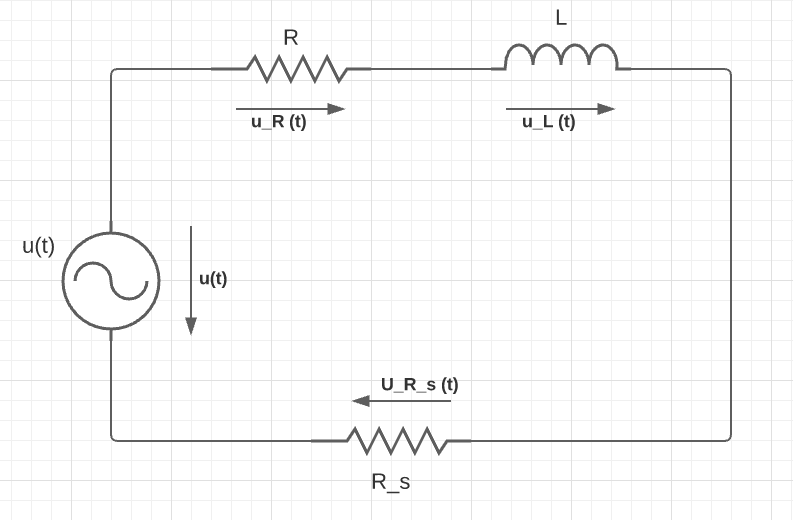
\includegraphics[width=1\textwidth]{schaltplan.png}
%     \caption{Mess-Schaltung Ankerinduktivität}
%     \label{fig:PlotAufgabe1}
%    \end{figure}

% Diese Schaltung kann durch folgende Maschengleichung beschrieben werden.

% \begin{equation} \label{eq211}
%     \begin{split}
%         u(t)&=u_R(t) + u_L(t)\\
%         u(t)&=R \cdot i(t) + L \frac{d i(t)}{dt}\\
%         u(t)&= (R+R_s) \cdot i(t) + L \frac{d i(t)}{dt}
%     \end{split}
% \end{equation}
